\begin{figure}[ht]
  \centering
    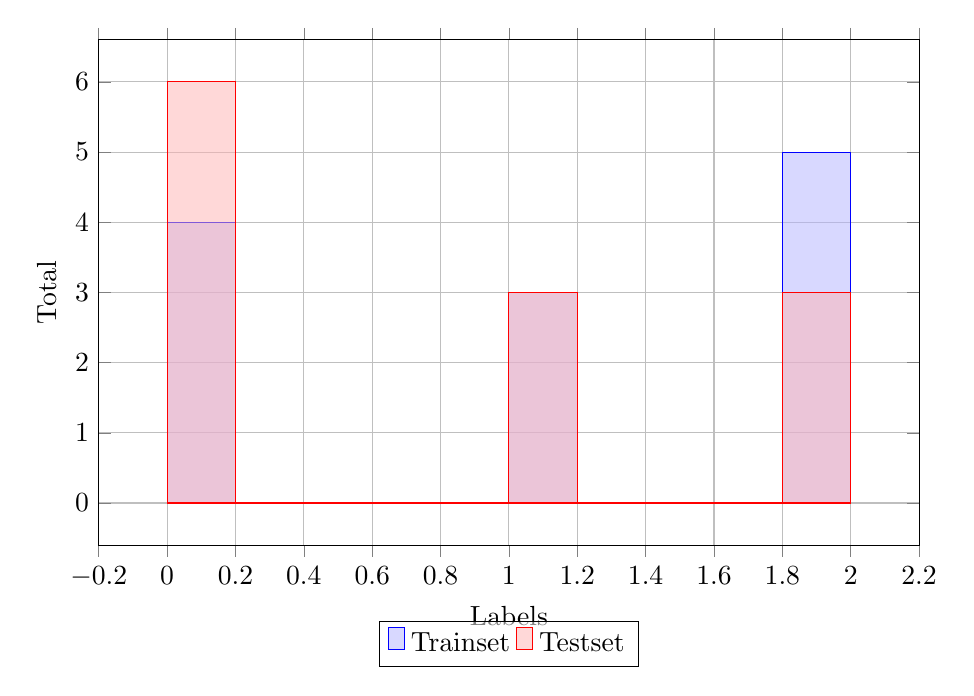
\begin{tikzpicture}
      \begin{axis}[
        xlabel=Labels,
        ylabel=Total,
        legend style={anchor=north, at={(0.5,-0.15)}, legend columns=-1},
        height=8cm,
        width=12cm,
        grid=both,
        ybar,
        text opacity=1,
        fill,
        fill opacity=0.5,
      ]
        \addplot+[hist={bins=10}]
          table[row sep=\\,y index=0] {
          data\\
          1\\
          2\\
          1\\
          0\\
          2\\
          2\\
          2\\
          2\\
          0\\
          1\\
          0\\
          0\\
          };
        \addplot+[hist={bins=10}]
          table[row sep=\\,y index=0] {
          data\\
          2\\
          2\\
          0\\
          1\\
          2\\
          0\\
          0\\
          0\\
          0\\
          1\\
          0\\
          1\\
          };
       \legend{ Trainset,Testset, }
     \end{axis}
    \end{tikzpicture}
  \caption{Dataset overview.}
\end{figure}
\begin{figure}[ht]
  \centering
    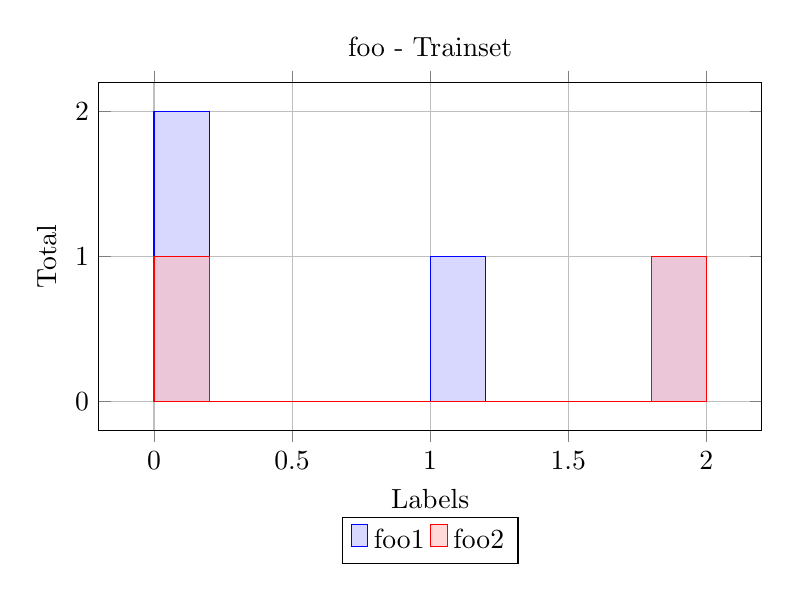
\begin{tikzpicture}
      \begin{axis}[
        title=foo - Trainset,
        name=foo,
        xlabel=Labels,
        ylabel=Total,
        legend style={anchor=north, at={(0.5,-0.25)}, legend columns=-1},
        height=6cm,
        width=10cm,
        grid=both,
        ybar,
        text opacity=1,
        fill,
        fill opacity=0.5,
        bar width=1
      ]
        \addplot+[hist={bins=10}]
          table[row sep=\\,y index=0] {
          data\\
          0\\
          2\\
          1\\
          0\\
          };
        \addplot+[hist={bins=10}]
          table[row sep=\\,y index=0] {
          data\\
          2\\
          0\\
          };
       \legend{ foo1,foo2, }
     \end{axis}
    \end{tikzpicture}
  \caption{Overview of foo over Train set.}
\end{figure}
\begin{figure}[ht]
  \centering
    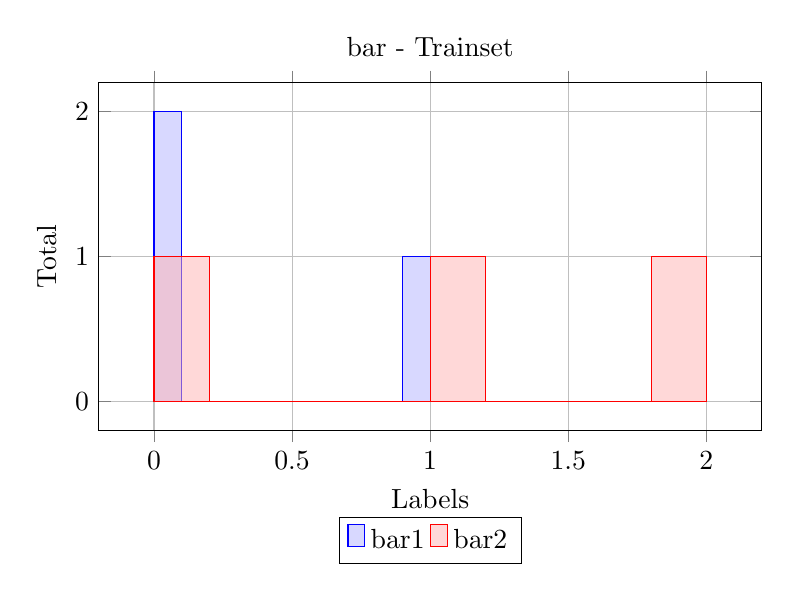
\begin{tikzpicture}
      \begin{axis}[
        title=bar - Trainset,
        name=bar,
        xlabel=Labels,
        ylabel=Total,
        legend style={anchor=north, at={(0.5,-0.25)}, legend columns=-1},
        height=6cm,
        width=10cm,
        grid=both,
        ybar,
        text opacity=1,
        fill,
        fill opacity=0.5,
        bar width=1
      ]
        \addplot+[hist={bins=10}]
          table[row sep=\\,y index=0] {
          data\\
          0\\
          0\\
          1\\
          };
        \addplot+[hist={bins=10}]
          table[row sep=\\,y index=0] {
          data\\
          0\\
          1\\
          2\\
          };
       \legend{ bar1,bar2, }
     \end{axis}
    \end{tikzpicture}
  \caption{Overview of bar over Train set.}
\end{figure}
\begin{figure}[ht]
  \centering
    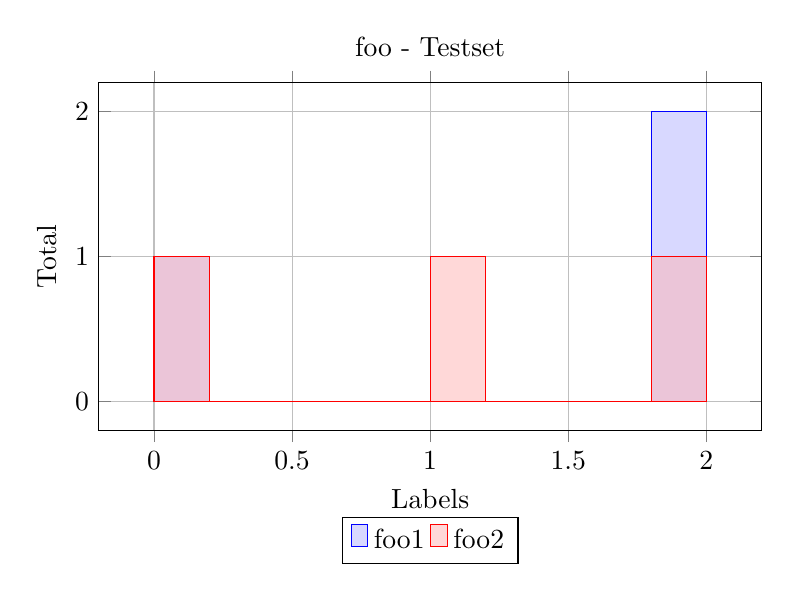
\begin{tikzpicture}
      \begin{axis}[
        title=foo - Testset,
        name=foo,
        xlabel=Labels,
        ylabel=Total,
        legend style={anchor=north, at={(0.5,-0.25)}, legend columns=-1},
        height=6cm,
        width=10cm,
        grid=both,
        ybar,
        text opacity=1,
        fill,
        fill opacity=0.5,
        bar width=1
      ]
        \addplot+[hist={bins=10}]
          table[row sep=\\,y index=0] {
          data\\
          0\\
          2\\
          2\\
          };
        \addplot+[hist={bins=10}]
          table[row sep=\\,y index=0] {
          data\\
          0\\
          1\\
          2\\
          };
       \legend{ foo1,foo2, }
     \end{axis}
    \end{tikzpicture}
  \caption{Overview of foo over Test set.}
\end{figure}
\begin{figure}[ht]
  \centering
    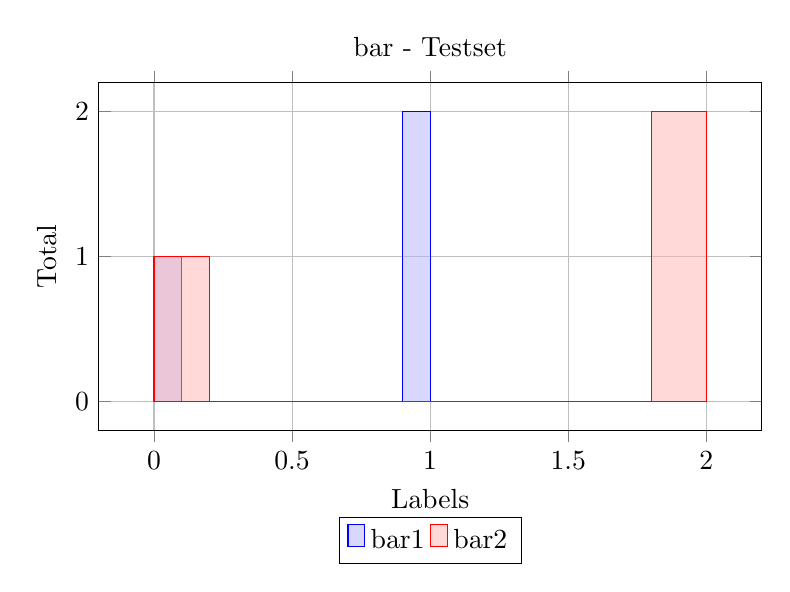
\begin{tikzpicture}
      \begin{axis}[
        title=bar - Testset,
        name=bar,
        xlabel=Labels,
        ylabel=Total,
        legend style={anchor=north, at={(0.5,-0.25)}, legend columns=-1},
        height=6cm,
        width=10cm,
        grid=both,
        ybar,
        text opacity=1,
        fill,
        fill opacity=0.5,
        bar width=1
      ]
        \addplot+[hist={bins=10}]
          table[row sep=\\,y index=0] {
          data\\
          0\\
          1\\
          1\\
          };
        \addplot+[hist={bins=10}]
          table[row sep=\\,y index=0] {
          data\\
          2\\
          2\\
          0\\
          };
       \legend{ bar1,bar2, }
     \end{axis}
    \end{tikzpicture}
  \caption{Overview of bar over Test set.}
\end{figure}
